\documentclass[12pt,fleqn]{article}\usepackage{common}
\begin{document}
Spline Egrileri

Diyelim ki elimizde 4 $y_i$ noktasi var, ve bu noktalardan gecen
yaklasiksal bir egri olusturmak istiyoruz. Spline yontemi her iki nokta
arasini farkli bir kupsel (ucuncu derece) polinom ile temsil
etmektir. Dikkat: farkli polinomlari toplamiyoruz, her aralikta baska bir
polinom fonksiyonu devreye giriyor. Peki niye kupsel? Cunku kupsel bir egri
yeterince kavis saglayabilir ve ayni zamanda cok fazla inisli cikisli
degildir.

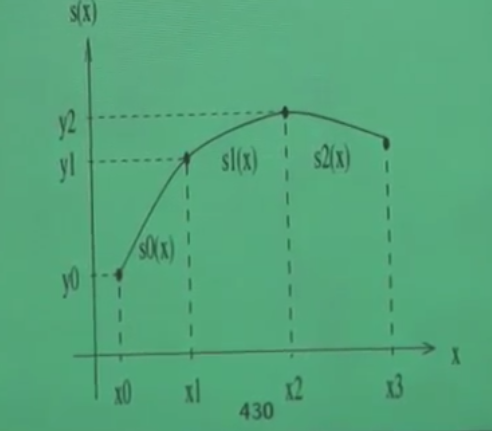
\includegraphics[height=4cm]{spline1.png}

Her $i=0,..,n-1$ icin 

\[ p(x) = s_i(x) = a_i + b_i(x-x_i) + c_i(x-x_i)^2 + d_i(x-x_i)^3
\ \ \ \label{1}
\]

kullanalim. Noktalar $x_i$ olarak gosteriliyor, ve her noktada aktif olan
bir $p_i$ spline olacak, o noktadan bir sonrakine kadar egriyi bu $s_i$
tanimlayacak. Peki her spline bir kubik polinom ise niye bu kubik polinomu
en basit sekliyle 

\[ p(x) = a_i + b_ix + c_ix^2 + d_ix^3 \]

olarak tanimlamadik? Cunku iki ustteki form ile calismak daha
rahat. Mesela, eger $x$ icin $x_i$ degrini verirsek, ki bu $x_1$ ya da
$x_2$ olabilirdi, o zaman parantez icinde $x_i - x_i$ sayesinde tum terimler sifir
oluyor, geriye sadece $a_i$ kaliyor. 

Parcalarin biraraya gelmesini nasil saglayacagiz? Bunun icin birkac sart
gerekli. Once en basit olani, bir onceki parca ile bir sonraki parcanin orta
nokta uzerinde ayni degere sahip olmasi. $i=1,..,n+1$ icin

\[ p_i (x_{i+1}) = p_{i+1}(x_{i+1}) \]

Tabii ki en basit gereklilik, her $x_i$'ye tekabul eden spline fonksiyonun
elimizdeki $y_i$ degerini vermesi,

\[ p_i(x_i) = y_i \]

Son parca bir istisna olusturuyor, o hem son nokta, hem de ondan bir onceki
nokta icin gecerli olmali

\[ p_{n-1}(x_n) = y_n \]

Teknigin isleyisini gelirsek, (1)'deki formulu ustteki gordugumuz her
$p_i(x)$'in yerine geciriyoruz. Bunu yapinca elimize bir lineer sistem
gececek, $4n$ tane denklem ve $4n$ tane bilinmez degiskenin oldugu bir
denklem sistemi olacak bu, ve boyle bir sistemin cozumu vardir. 

Simdi indisleri degistirelim, ve $i=1,..,n+1$ olarak tasarlayalim. Tum
denklemleri yazarsak,

\[ p_1(x) = s_1(x) = a_1 + b_1(x-x_1) + c_1(x-x_1)^2 + d_1(x-x_1)^3\]

\[ p_2(x) = s_2(x) = a_2 + b_2(x-x_2) + c_2(x-x_2)^2 + d_1(x-x_2)^3\]

\[ \vdots \]

\[ p_3(x) = s_3(x) = a_3 + b_3(x-x_3) + c_3(x-x_2)^2 + d_3(x-x_2)^3\]

Uc noktali soyle bir grafik dusunelim,

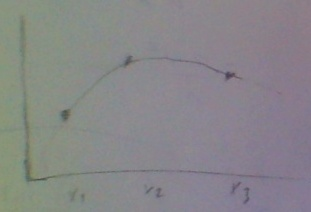
\includegraphics[height=4cm]{spline2.png}

Ustte bahsettigimiz gibi, $p_1(x_1) = a_1 = y_1$ olacak, ve tum indisler
icin bu gecerli. Ayrica $x_2$ noktasinda bir onceki parca ve sonraki parca
ayni degere sahip olmali demistik, yani mesela $p_1$'in sonunda (ustteki
ilk parca) $x_2$ noktasi vardir, ve ayni noktada $p_2$ baslayacaktir, o
noktada 

\[ p_1(x_2) = a_1 + b_1h_1 + c_1h_1^2 + d_1h_1^3  \]

ve bu denklem $p_2(x_2) = a_2 = y_2$'ye esit. Ayrica daha once gorduk, $a_1 =
y_1$ 
ise, o zaman 

\[ y_2 = p_1(x_2) = a_1 + b_1h_1 + c_1h_1^2 + d_1h_1^3 \]

haline gelir. Kisaca

\[ y_2 =  y_1 + b_1h_1 + c_1h_1^2 + d_1h_1^3 \]

Hepsini birarada yaziyoruz, tek basina olan $y$'yi sag tarafa aliyoruz

\[ y_1 + b_1h_1 + c_1h_1^2 + d_1h_1^3 = y_2 \]

\[ y_2 + b_2h_2 + c_2h_2^2 + d_2h_2^3 = y_3 \]

\[ \vdots \]

\[ y_n + b_nh_n + c_nh_n^2 + d_nh_n^3 = y_n \]

ki $h_1 \equiv x_2 - x_1$, $h_2 \equiv x_3 - x_2$ olarak tanimlandi. Yani bir tur kisaltma 
olarak $h$ harfini kullaniyoruz. 














http://spartan.ac.brocku.ca/~jvrbik/MATH2P20/notes.pdf

http://www.youtube.com/watch?v=3rHBCglD1LQ

http://www.youtube.com/watch?v=nA0YpqraP9A


\end{document}
